\documentclass{ximera}

\title{Intro to Derivatives Activity}
\author{MATH 425: Calculus I}

\begin{document}
\begin{abstract}
    Working with the peers in your group, solve the following problems. Make sure to show and justify all your work. Make sure everyone in the group understands the solution and participates. Be prepared to report your answers to the whole class. 
\end{abstract}
\maketitle

\begin{definition}
        \textbf{The limit definition of the derivative}\\
        Suppose $f$ is a continuous function and $a$ is a value in the domain of $f$. The \textbf{derivative} of $f$ at $a$, denoted by $f'(a)$, is defined by the following limit (if it exists):
        $$f'(a)=\lim_{h\rightarrow 0}\frac{f(a+h)-f(a)}{h}\,\,\,\,\,\,\,\,\text{or}\,\,\,\,\,\,\,\,\,\,\,f'(a)=\lim_{b\rightarrow a}\frac{f(b)-f(a)}{b-a}$$
\end{definition}

\begin{exercise}
    Use the graph of $f(x)$ below to evaluate the requested derivative values.
    \begin{image}
        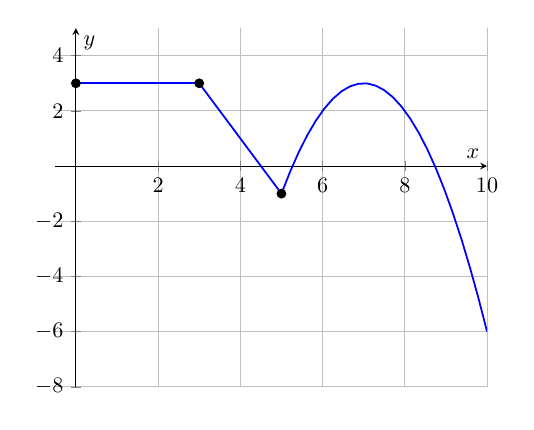
\begin{tikzpicture}[scale=0.8]
            \begin{axis}[
                xlabel=$x$,
                ylabel=$y$,
                axis lines=middle,
                grid=major,
                xmin=-0.5, xmax=10,
                ymin=-8, ymax=5,
            ]
            
            % y=3 from x=0 to x=3
            \addplot[blue, thick, domain=0:3] {3};
            
            % y=-2x+9 from x=3 to x=5
            \addplot[blue, thick, domain=3:5] {-2*x+9};
            
            % y=-(x-7)^2+3 from x=5 on
            \addplot[blue, thick, domain=5:10] {-(x-7)^2+3};
            
            % Mark endpoints
            \addplot[only marks, mark=*] coordinates {(0,3) (3,3) (5,-1)};
            
            \end{axis}
        \end{tikzpicture}
    \end{image}
    %\xmalt Graph of a piecewise function on the domain $[0,\infty)$: defined by $y=3$ when $0\leq x\leq 3$, $y=-2x+9$ when $3<x<5$ and $y=-(x-7)^2+3$ when $5\leq x$.
    \begin{enumerate}
        \item $f'(1)$ \textcolor{blue}{$=3$}
        \item $f'(2)$ \textcolor{blue}{$=3$}
        \item $f'(4)$ \textcolor{blue}{$=-2$}
        \item $f'(7)$ \textcolor{blue}{$=0$}
    \end{enumerate}
\end{exercise}

\begin{exercise}
Calculate the following derivatives at the given value using both the $h\rightarrow 0$ and $b\rightarrow a$ limit definitions of the derivative.\\
    \begin{enumerate}
        \item $f(x)=3x+2$ at $a=1$\\
        \textcolor{blue}{Using $b\rightarrow a$:\\
        $\displaystyle f'(1)=\lim_{b\rightarrow 1}\frac{3b+2-5}{b-1}=\lim_{b\rightarrow 1}\frac{3(b-1)}{b-1}=3$\\
        Using $h\rightarrow 0$:\\
        $\displaystyle f'(1)=\lim_{h\rightarrow 0}\frac{3(1+h)+2-5}{h}=\lim_{h\rightarrow 0}\frac{3+3h-3}{h}=\lim_{h\rightarrow 0}\frac{3h}{h}=3$}
        
        \item $f(x)=x^2-3x$ at $a=-1$\\
        \textcolor{blue}{ Using $b\rightarrow a$:\\
        $\displaystyle f'(-1)=\lim_{b\rightarrow -1}\frac{b^2-3b-4}{b+1}=\lim_{b\rightarrow -1}\frac{(b-4)(b+1)}{b+1}=\lim_{b\rightarrow -1}(b-4)=-5$\\
        Using $h\rightarrow 0$:\\
        $\displaystyle f'(-1)=\lim_{h\rightarrow 0}\frac{(-1+h)^2-3(-1+h)-4}{h}=\lim_{h\rightarrow 0}\frac{1-2h+h^2+3-3h-4}{h}=\lim_{h\rightarrow 0}\frac{-5h+h^2}{h}$\\
        $=\lim_{h\rightarrow 0}-5+h=-5$}
        
        \item $f(x)=x^3-4$ at $a=0$.\\
        \textcolor{blue}{Using $b\rightarrow a$:\\
        $\displaystyle f'(0)=\lim_{b\rightarrow 0}\frac{b^3-4+4}{b}=\lim_{b\rightarrow 0}\frac{b^3}{b}=\lim_{b\rightarrow 0}b^2=0$\\
        Using $h\rightarrow 0$:\\
        $\displaystyle f'(0)=\lim_{h\rightarrow 0}\frac{(h)^3-4+4}{h}=\lim_{h\rightarrow 0}\frac{h^3}{h}=\lim_{h\rightarrow 0}h^2=0$}
        
        \item Did either version of the derivative definition seem easier to use or more helpful?  For which functions? 
    \end{enumerate}

    \end{exercise}

    \begin{exercise} 
        \begin{enumerate}
            \item Find the equation to the tangent line to $f(x)=x^2-3x$ at $a=-1$.\\
            \textcolor{blue}{$f'(-1)=-5$ (calculated in 1b)\\
                $f(-1)=(-1)^2-3(-1)=4$\\
                Equation of the tangent line: $y-4=-5(x+1)$}
            \item Find the equation to the tangent line to $f(x)=x^2-3x$ at $a=2$.\\
            \textcolor{blue}{$f'(2)=\displaystyle\lim_{h\rightarrow 0}\frac{(2+h)^2-3(2+h)+2}{h}=\lim_{h\rightarrow 0}\frac{4+2h+h^2-6-3h+2}{h}=\lim_{h\rightarrow 0}\frac{-h+h^2}{h}=\lim_{h\rightarrow 0}\frac{h(-1+h)}{h}$\\
            $=\displaystyle \lim_{h\rightarrow 0} -1+h=-1$\\
            $f(2)=2^2-3(2)=-2$\\
            Equation of the tangent line: $y+2=-(x-2)$}
        \end{enumerate}
    \end{exercise}

    \begin{exercise}
        Show that the derivative of the function $f(x)=x^{1/3}$ does not exist at $a=0$.\\
        \textcolor{blue}{$f'(0)=\displaystyle\lim_{h\rightarrow 0} \frac{h^{1/3}-0}{h}=\lim_{h\rightarrow 0}\frac{1}{h^{2/3}}=\infty$ (The 2/3 power means to take a cube root and square the value, so the numerator will always be positive.) \\
        Since the limit does not exist (is not finite), the derivative doesn't exist.}
    \end{exercise}
   

    \begin{exercise}
    
    Let $f(x)=2x^2-3x+5$. Show that the secant line through $(2,f(2))$  and $(2+h, f(2+h))$ has slope $2h+5$. Then use this formula to compute:
    \begin{enumerate}
        \item The slope of the secant line through $(2,f(2))$  and $(3,f(3))$ \\
        \textcolor{blue}{$2+h=3$, so $h=1$\\
        $m=2(1)+5=7$}
        
         \item The slope of the tangent line at $a=2$  (by taking a limit)\\
         \textcolor{blue}{$m=\lim_{h\rightarrow 0}2h+5=5$}
        
         \item The slope of the tangent line at $a=2$ using the limit definition of the derivative. (Your answers to b and c should match).\\
         \textcolor{blue}{$f'(2)=\displaystyle\lim_{h\rightarrow 0}\frac{2(2+h)^2-3(2+h)+5-7}{h}=\lim_{h\rightarrow0}\frac{8+8h+2h^2-6-3h+5-7}{h}=\lim_{h\rightarrow0}\frac{5h+2h^2}{h}$\\
         $=\displaystyle\lim_{h\rightarrow0}5+2h=5$}
         
         (Adapted from Rogawski et al, \textit{Calculus: Early Transcendentals}, 4th ed.)
    \end{enumerate}
    \end{exercise} 

    \begin{exercise}
        The graph of $f(x)$ is given below.
        \begin{image}
            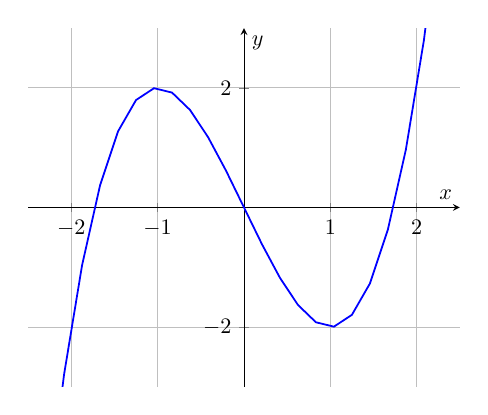
\begin{tikzpicture}[scale=0.8]
                \begin{axis}[
                    xlabel=$x$,
                    ylabel=$y$,
                    axis lines=middle,
                    grid=major,
                    xmin=-2.5, xmax=2.5,
                    ymin=-3, ymax=3,
                ]
                
                \addplot[blue, thick, domain=-2.5:2.5] {x^3-3*x};
                
                \end{axis}
            \end{tikzpicture}
        \end{image}
        %\xmalt Graph of $y=x^3-3x$.
        When is the derivative $f'(x)$:
        \begin{enumerate}
            \item positive? \textcolor{blue}{$x<-1$ and $x>1$}
            \item negative? \textcolor{blue}{$-1<x<1$}
            \item zero? \textcolor{blue}{at $x=-1,1$}
        \end{enumerate}
    \end{exercise}



\end{document}
